\begin{figure*}
        \centering
        \begin{subfigure}[b]{0.475\textwidth}
            \centering
            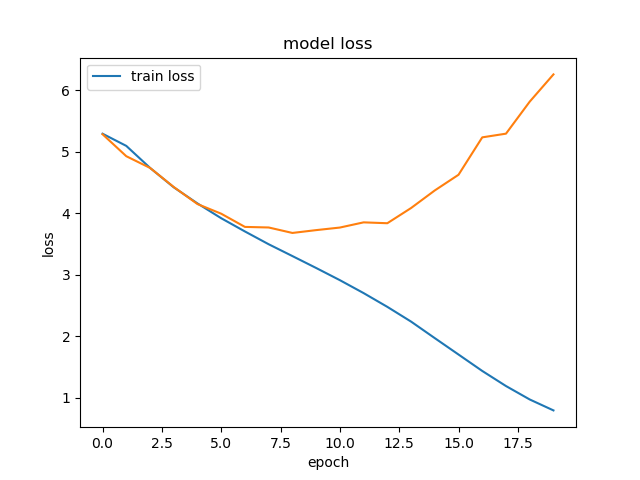
\includegraphics[width=\textwidth]{../images/run1_loss_a.png}
            \caption[]%
            {{\small }}
        \end{subfigure}
        \hfill
        \begin{subfigure}[b]{0.475\textwidth}
            \centering
            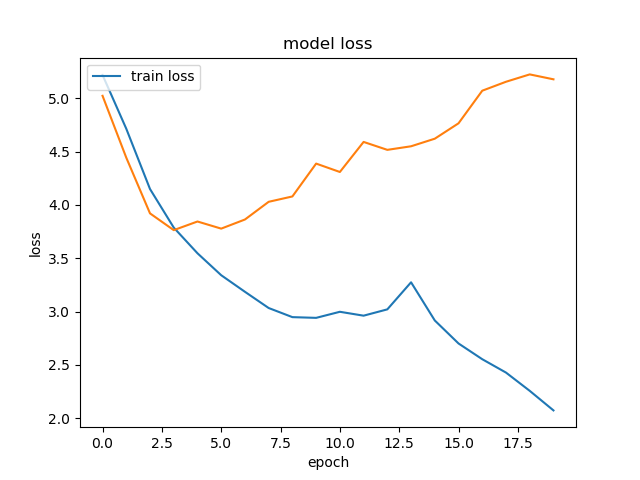
\includegraphics[width=\textwidth]{../images/run1_loss_b.png}
            \caption[]%
            {{\small }}
        \end{subfigure}
        \vskip\baselineskip
        \begin{subfigure}[b]{0.475\textwidth}
            \centering
            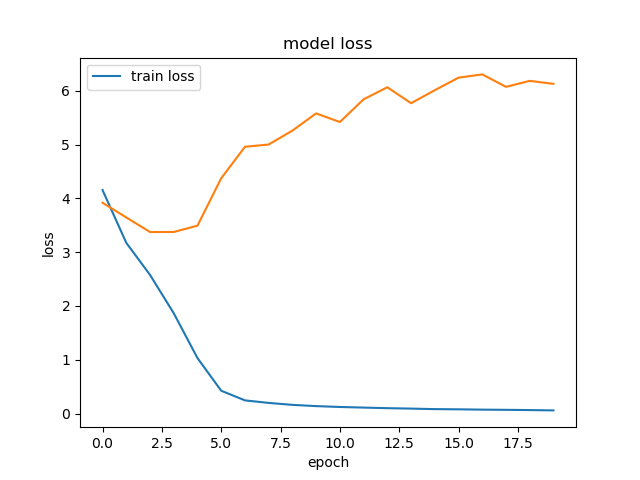
\includegraphics[width=\textwidth]{../images/run1_loss_c.png}
            \caption[]%
            {{\small }}
        \end{subfigure}
        \quad
        \begin{subfigure}[b]{0.475\textwidth}
            \centering
            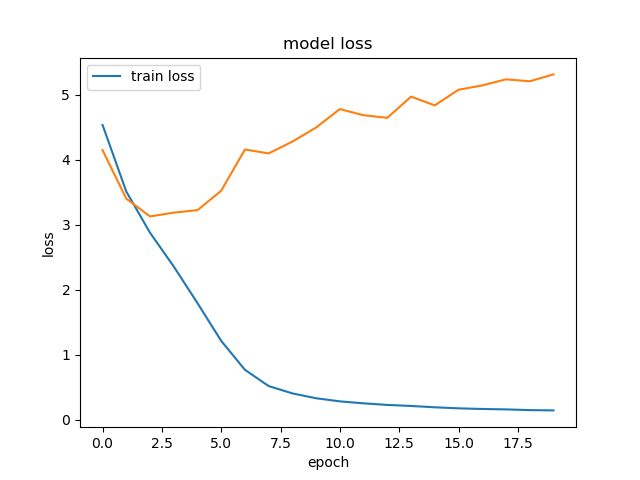
\includegraphics[width=\textwidth]{../images/run1_loss_d.png}
            \caption[]%
            {{\small }}
        \end{subfigure}
        \caption[]
        {\small Training and validation loss of 20 first epochs of respective models presented in table \ref{table:3_configurations}. Each suffer from immense overfitting 5-10 epochs of training.}
        \label{fig:4_losses}
    \end{figure*}
